\documentclass[11pt,a4paper]{article}
\usepackage[margin=23mm,headheight=15pt]{geometry}
\usepackage{fontspec}
\setmainfont{Times New Roman}
\setsansfont{Arial}
\usepackage{amsmath,amssymb,graphicx,booktabs,array,tabularx,longtable,caption,xcolor,fancyhdr,enumitem,placeins}
\usepackage[numbers,sort&compress]{natbib}
\usepackage[colorlinks=true,linkcolor=teal!55!black,citecolor=teal!55!black,urlcolor=teal!55!black]{hyperref}
\definecolor{navy}{HTML}{193447}
\definecolor{pale}{HTML}{EDF4F5}
\usepackage{titlesec}
\titleformat{\section}{\large\sffamily\bfseries\color{navy}}{}{0em}{}
\setlength{\parindent}{0pt}
\setlength{\parskip}{6pt}
\raggedbottom
\setlength{\emergencystretch}{3em}
\widowpenalty=10000\clubpenalty=10000
\renewcommand{\topfraction}{.95}\renewcommand{\bottomfraction}{.85}\renewcommand{\textfraction}{.05}\renewcommand{\floatpagefraction}{.75}
\renewcommand{\arraystretch}{1.16}
\captionsetup{font=small,labelfont=bf,justification=raggedright,singlelinecheck=false}
\pagestyle{fancy}\fancyhf{}\fancyhead[L]{\small\sffamily EVIDENCE TO EXPERIMENT}\fancyhead[R]{\small\sffamily 18 November 2026}\fancyfoot[C]{\thepage}
\renewcommand{\headrulewidth}{0.3pt}
\graphicspath{{figures/}}
\newcounter{boxnum}
\newcommand{\boxlabel}{Box}
\begin{document}
{\small\sffamily\color{navy} SUPPLEMENTARY EVIDENCE ATLAS}\par\medskip
{\LARGE\bfseries\raggedright Evidence map and experiment-selection rules\par}\bigskip
{\normalsize JiaHao Wu and Long Zeng\par}
{\small Tsinghua Shenzhen International Graduate School, Tsinghua University, Shenzhen, China\par}\medskip
\hypersetup{pdfauthor={JiaHao Wu; Long Zeng}}
{\small Correspondence: Long Zeng, \href{mailto:zenglong@sz.tsinghua.edu.cn}{zenglong@sz.tsinghua.edu.cn}\par}\medskip
The 29 entries distinguish published observations from our interpretive synthesis and proposed tests. Each entry cites the source and a figure, experiment or section locator. The eight decision cards specify controls and computational boundaries. Coverage is centered on human upper-limb adaptation; the 2026 reviewed preprint and computational contributions are explicitly labelled. The full paired records are also supplied as JSON.
\begin{table}[!htbp]\small\caption{From established findings to the experimental increment of this synthesis. The first column credits prior contributions; the next columns state the joint interpretation and the comparison it motivates.}\label{tab:synthesis}
\begin{tabularx}{\textwidth}{>{\raggedright\arraybackslash}X>{\raggedright\arraybackslash}X>{\raggedright\arraybackslash}X}\toprule
\textbf{Established contribution} & \textbf{Joint interpretation} & \textbf{Experimental consequence}\\\midrule
Sensory-specific memories combine at output (Hayashi et al.). & Separate acquisition can support transfer into several control outputs. & Cross sensory error channels with anticipatory and corrective readouts.\\[6pt]
Adaptation contains interacting timescales (Smith et al.). & Fixed mixed readout can generate delay-dependent dissociation. & Predict both outputs at reserved delays; compare common and output-specific dynamics.\\[6pt]
Context affects updating and expression (Heald et al.). & Transfer depends on both the training condition and the condition of measurement. & Cross training and test cues; use the first error-free probe at matched delay.\\[6pt]
Active and passive localization sample different information (Gastrock et al.). & A report constrains input versus updating through its component loadings. & Calibrate report loadings independently and predict joint report-and-motor outcomes.\\[6pt]
\bottomrule\end{tabularx}\end{table}
\section{Reading the evidence levels}
Observed result: what the experiment measured. Supported inference: the mechanism level constrained by its controls. Residual explanation: a specific alternative that can produce the observation. Proposed test: our next comparison and its predicted interpretive value. A surviving alternative is retained without changing the original result.
\clearpage\section{E01 | Shared Internal Models for Feedforward and Feedback Control}
{\small\sffamily\color{navy} Transfer}\par
\textbf{Source} \cite{wagner2008}; Results: responses to unexpected perturbations after force-field learning; model comparisons\par
\textbf{Study type / status} Published primary study\par
\textbf{Manipulation and comparison} Train reaches in altered dynamics, then introduce unexpected perturbations during movement.\par
\textbf{Measured outcome} Time-resolved corrective responses and trajectories across learned dynamics.\par
\textbf{Observed finding} Corrections incorporated knowledge acquired during force-field training.\par
\textbf{Supported inference} Learned dynamics influence both planned and corrective behaviour.\par
\textbf{Residual explanation} A shared dynamics estimate and a trained recurrent policy can both carry knowledge into corrective behaviour.\par
\textbf{Discriminating prediction / proposed addition} Hold baseline trajectories constant; predict untrained perturbation directions and timings with parameters fixed before testing.\par
\bigskip\hrule\medskip\section{E02 | Feedforward and Feedback Control Share an Internal Model of the Arm's Dynamics}
{\small\sffamily\color{navy} Transfer}\par
\textbf{Source} \cite{maeda2018}; Figures 3, 6 and 7; shoulder-fixation and no-fixation control\par
\textbf{Study type / status} Published primary study\par
\textbf{Manipulation and comparison} Fix the shoulder during voluntary elbow reaches; test mechanical perturbations with the shoulder free.\par
\textbf{Measured outcome} Shoulder EMG in reaching and in the 50--100 ms long-latency response; pre-perturbation EMG and elbow-muscle controls.\par
\textbf{Observed finding} Reduced shoulder activation during learning transferred to long-latency shoulder responses.\par
\textbf{Supported inference} Transfer reaches a rapid feedback pathway, with baseline activation controls.\par
\textbf{Residual explanation} Shared storage, coupled updates and common task-dependent readout remain candidate implementations.\par
\textbf{Discriminating prediction / proposed addition} Cross training and test contexts while measuring pre-perturbation EMG and short- and long-latency responses.\par
\clearpage\section{E03 | Learning New Feedforward Motor Commands Based on Feedback Responses}
{\small\sffamily\color{navy} Transfer}\par
\textbf{Source} \cite{maeda2020}; Figures 3--4; perturbation training and transfer-to-reaching probes\par
\textbf{Study type / status} Published primary study\par
\textbf{Manipulation and comparison} Train responses to mechanical perturbations with shoulder fixation and reduced voluntary intervention; probe voluntary reaches.\par
\textbf{Measured outcome} Long-latency shoulder responses during training and anticipatory shoulder EMG in reach probes.\par
\textbf{Observed finding} Feedback training altered subsequent voluntary motor commands.\par
\textbf{Supported inference} Transfer can operate from feedback training to voluntary control, complementing the reverse direction.\par
\textbf{Residual explanation} Bidirectional transfer is compatible with common representations or communication between distinct representations.\par
\textbf{Discriminating prediction / proposed addition} Measure transfer after a matched delay in both directions; compare adaptation and retention under identical probe contexts.\par
\bigskip\hrule\medskip\section{E04 | Structural learning in feedforward and feedback control}
{\small\sffamily\color{navy} Dissociation}\par
\textbf{Source} \cite{yousif2012}; Experiments 1--3; Figures 4--6, especially Figure 6\par
\textbf{Study type / status} Published primary study\par
\textbf{Manipulation and comparison} Change the temporal consistency of position-dependent force exposure while matching counts of field, null and channel trials.\par
\textbf{Measured outcome} Position/velocity components of channel forces in feedforward adaptation and feedback to target--channel misalignment.\par
\textbf{Observed finding} Consistent exposure changed both domains; inconsistent exposure changed feedback structure without the corresponding feedforward structural change.\par
\textbf{Supported inference} Temporal statistics condition the coupling between the measured control outputs.\par
\textbf{Residual explanation} Different update rules, timescales or context-dependent expression can create this dissociation.\par
\textbf{Discriminating prediction / proposed addition} Add common-context probes at multiple delays; persistence under matched readout favours a learning/retention difference over immediate gating.\par
\clearpage\section{E05 | Learning feedback and feedforward control in a mirror-reversed visual environment}
{\small\sffamily\color{navy} Dissociation}\par
\textbf{Source} \cite{kasuga2015}; Figures 3--5; endpoint, online and no-mirror control groups\par
\textbf{Study type / status} Published primary study\par
\textbf{Manipulation and comparison} Train mirror-reversed reaching with endpoint-only or continuous visual feedback.\par
\textbf{Measured outcome} Initial movement direction and force responses to cursor jumps; principal response window 251--350 ms.\par
\textbf{Observed finding} Endpoint feedback favoured feedforward performance; online exposure produced greater attenuation of inappropriate feedback responses.\par
\textbf{Supported inference} Exposure to online consequences matters for acquiring a changed feedback policy.\par
\textbf{Residual explanation} Mirror reversal requires policy remapping; training duration and sensory exposure differ from force-field adaptation.\par
\textbf{Discriminating prediction / proposed addition} Match exposure and asymptotic baseline performance, then compare full response waveforms across training duration.\par
\bigskip\hrule\medskip\section{E06 | The Neural Feedback Response to Error As a Teaching Signal for the Motor Learning System}
{\small\sffamily\color{navy} Teaching signal}\par
\textbf{Source} \cite{albert2016}; Figures 1, 5--6; 2016 correction concerns Figure 2A Error 2 displacement traces\par
\textbf{Study type / status} Published primary study\par
\textbf{Manipulation and comparison} Place one or two curl-field trials between baseline and post-error channel trials.\par
\textbf{Measured outcome} Perturbation-minus-baseline EMG and post-error-minus-baseline EMG across muscles.\par
\textbf{Observed finding} Learning-related EMG resembled a scaled corrective response advanced by about 125 ms.\par
\textbf{Supported inference} The observed muscle patterns support a feedback-related teaching signal in this force-field paradigm.\par
\textbf{Residual explanation} A shared upstream error drive can couple the signals; temporal copying requires additional timing manipulations.\par
\textbf{Discriminating prediction / proposed addition} Shift perturbation onset and reverse late error while pairing correction and next-trial force/EMG; predict timing as well as amplitude.\par
\clearpage\section{E07 | Tonic feedback motor commands predict visuomotor learning}
{\small\sffamily\color{navy} Teaching signal}\par
\textbf{Source} \cite{makino2026}; Experiments 1--3; Figures 1--4; reviewed preprint v1, 29 June 2026\par
\textbf{Study type / status} Reviewed preprint, version 1\par
\textbf{Manipulation and comparison} Manipulate onset, magnitude and temporal pattern of cursor displacement within a force channel.\par
\textbf{Measured outcome} Baseline-subtracted corrective force and next-trial learning force, including the terminal holding period.\par
\textbf{Observed finding} Learning onset remained linked to movement onset; tonic holding responses predicted learning amplitude across changed visual-error patterns.\par
\textbf{Supported inference} Visual-error timing constrains a universal fixed-time-shift copying account.\par
\textbf{Residual explanation} Tonic force may index an integrated teaching variable; causal mediation and transfer to force-field errors remain open.\par
\textbf{Discriminating prediction / proposed addition} Use matched visual and mechanical temporal perturbations; compare prespecified copying and temporal-integration models on held-out onset patterns.\par
\bigskip\hrule\medskip\section{E08 | Rapid Feedback Responses Correlate with Reach Adaptation and Properties of Novel Upper Limb Loads}
{\small\sffamily\color{navy} Transfer}\par
\textbf{Source} \cite{cluff2013}; Results: load magnitude/direction and rapid-feedback adaptation\par
\textbf{Study type / status} Published primary study\par
\textbf{Manipulation and comparison} Adapt reaches to novel upper-limb loads with different magnitudes and directions.\par
\textbf{Measured outcome} Reach adaptation and rapid perturbation-evoked muscle responses at a probe target with controlled background activation.\par
\textbf{Observed finding} Feedback changes covaried with reach adaptation and properties of the learned load.\par
\textbf{Supported inference} Feedback modulation carries load-specific information.\par
\textbf{Residual explanation} The background-activation control constrains automatic gain scaling; common estimates and jointly trained outputs remain alternative implementations.\par
\textbf{Discriminating prediction / proposed addition} Measure gain scaling at matched background activation and test unseen load--target combinations.\par
\clearpage\section{E09 | Adaptation to Stable and Unstable Dynamics Achieved By Combined Impedance Control and Inverse Dynamics Model}
{\small\sffamily\color{navy} Mechanics}\par
\textbf{Source} \cite{franklin2003}; Stable velocity field versus unstable divergent field; Figures 5--10\par
\textbf{Study type / status} Published primary study\par
\textbf{Manipulation and comparison} Compare adaptation to stable velocity-dependent and unstable divergent dynamics.\par
\textbf{Measured outcome} Trajectory, force/torque and muscle activation across learning.\par
\textbf{Observed finding} Successful adaptation combined changes in compensatory commands and coactivation, depending on environmental stability.\par
\textbf{Supported inference} Body mechanics contribute to similar improvements in trajectory accuracy.\par
\textbf{Residual explanation} EMG coactivation is an indirect stiffness measure; neural feedback and intrinsic mechanics both influence resistance.\par
\textbf{Discriminating prediction / proposed addition} Add small multidirectional mechanical probes, background EMG and latency-resolved force to estimate impedance independently.\par
\bigskip\hrule\medskip\section{E10 | Visuomotor feedback tuning in the absence of visual error information}
{\small\sffamily\color{navy} Dissociation}\par
\textbf{Source} \cite{franklin2023}; Results: visual-error availability, feedback gains and co-contraction\par
\textbf{Study type / status} Published primary study\par
\textbf{Manipulation and comparison} Vary abrupt/gradual force-field introduction and availability of visual trajectory error.\par
\textbf{Measured outcome} Adaptation, visuomotor feedback gains and co-contraction.\par
\textbf{Observed finding} Removing visual error reduced feedback gains while preserving their learning-related modulation pattern.\par
\textbf{Supported inference} A measured visual gain depends on sensory conditions as well as training state.\par
\textbf{Residual explanation} Uncertainty-based interpretations require a separate estimate of uncertainty.\par
\textbf{Discriminating prediction / proposed addition} Calibrate visual reliability and correction gain outside learning, then predict transfer across the reliability manipulation.\par
\clearpage\section{E11 | Feedback Adaptation to Unpredictable Force Fields in 250 ms}
{\small\sffamily\color{navy} Timescale}\par
\textbf{Source} \cite{crevecoeur2020}; Experiments 1--2; Figures 3--7\par
\textbf{Study type / status} Published primary study\par
\textbf{Manipulation and comparison} Present unanticipated force fields in a random sequence, including different field types.\par
\textbf{Measured outcome} Within-reach EMG, force and late movement kinematics.\par
\textbf{Observed finding} Feedback became tuned to the ongoing field on a timescale of roughly 250 ms from reach onset.\par
\textbf{Supported inference} Adaptation-related adjustment can operate within an ongoing movement.\par
\textbf{Residual explanation} Fast identification and selection among available policies can produce related within-trial changes.\par
\textbf{Discriminating prediction / proposed addition} Probe the next trial after matched within-trial corrections; test whether the change persists and generalizes.\par
\bigskip\hrule\medskip\section{E12 | Learning from Sensory and Reward Prediction Errors during Motor Adaptation}
{\small\sffamily\color{navy} Readout}\par
\textbf{Source} \cite{izawa2011}; Sensory versus reward prediction-error training; sensory remapping and generalization results\par
\textbf{Study type / status} Published primary study\par
\textbf{Manipulation and comparison} Compare training driven by sensory prediction error with reward-based learning.\par
\textbf{Measured outcome} Motor adaptation together with reported sensory consequences and generalization.\par
\textbf{Observed finding} The learning routes produced distinguishable sensory remapping despite changes in motor performance.\par
\textbf{Supported inference} A paired perceptual readout constrains which internal consequences accompany learning.\par
\textbf{Residual explanation} Perceptual reports depend on task, estimation and response mapping.\par
\textbf{Discriminating prediction / proposed addition} Add passive and active localization with identical report mappings and matched movement performance.\par
\clearpage\section{E13 | Estimating the sources of motor errors for adaptation and generalization}
{\small\sffamily\color{navy} Source attribution}\par
\textbf{Source} \cite{berniker2008}; Model and comparisons with published generalization experiments; Figures 1--5\par
\textbf{Study type / status} Computational theory with comparisons to prior experiments\par
\textbf{Manipulation and comparison} Model latent changes in body and external-world dynamics and compare predicted transfer with published experiments.\par
\textbf{Measured outcome} Predicted generalization across workspace, limbs and object contexts.\par
\textbf{Observed finding} Different inferred disturbance sources produced different patterns of generalization.\par
\textbf{Supported inference} Source inference supplies a computational account of structured generalization.\par
\textbf{Residual explanation} The fit of a source-estimation model supports explanatory sufficiency; competing latent-state models may share predictions.\par
\textbf{Discriminating prediction / proposed addition} Change source cues at matched physical errors and preregister predictions for an untrained limb or object.\par
\bigskip\hrule\medskip\section{E14 | Relevance of Error: What Drives Motor Adaptation?}
{\small\sffamily\color{navy} Source attribution}\par
\textbf{Source} \cite{wei2009}; Experiments manipulating error magnitude; relevance model\par
\textbf{Study type / status} Published primary study\par
\textbf{Manipulation and comparison} Vary sensory error magnitude in reaching adaptation.\par
\textbf{Measured outcome} Trial-to-trial adaptation as a function of error size.\par
\textbf{Observed finding} Error sensitivity varied nonlinearly with error magnitude, motivating an estimate of error relevance.\par
\textbf{Supported inference} Learning gain depends on more than physical error magnitude alone.\par
\textbf{Residual explanation} Saturating encodings and changing beliefs can yield related input--output curves.\par
\textbf{Discriminating prediction / proposed addition} Cross error magnitude with independently manipulated source credibility; measure perceived error as well as learning.\par
\clearpage\section{E15 | External error attribution dampens efferent-based predictions but not proprioceptive changes in hand localization}
{\small\sffamily\color{navy} Source attribution}\par
\textbf{Source} \cite{external2020}; Results: reach aftereffects, passive localization, active-minus-passive localization; hand-view and cursor-jump groups\par
\textbf{Study type / status} Published primary study\par
\textbf{Manipulation and comparison} Expose a visuomotor rotation through a visible cursor jump or direct hand view.\par
\textbf{Measured outcome} Reach aftereffects, passive localization and active-minus-passive localization.\par
\textbf{Observed finding} Aftereffects were reduced in the exposure groups. Passive localization shifts persisted; the hand-view active-minus-passive estimate was near zero, while its direct contrast with control remained uncertain.\par
\textbf{Supported inference} Motor aftereffects and report components show different response patterns; the hand-view contrast does not uniquely identify elimination of an efferent mechanism.\par
\textbf{Residual explanation} Hand view changes sensory information together with attribution; active-minus-passive localization depends on subtraction assumptions.\par
\textbf{Discriminating prediction / proposed addition} Add a credible cue-only attribution condition with identical hand visibility and independently calibrated localization.\par
\bigskip\hrule\medskip\section{E16 | Causal inference, prediction and state estimation in sensorimotor learning}
{\small\sffamily\color{navy} Source attribution}\par
\textbf{Source} \cite{piece2025}; Figure 1 experimental setup; Figure 2 human results; model comparisons\par
\textbf{Study type / status} Published primary study\par
\textbf{Manipulation and comparison} Compare small externally imposed rotations with internally generated movement variability matched in scale.\par
\textbf{Measured outcome} Subsequent trial-to-trial angular change relative to the error trial.\par
\textbf{Observed finding} Participants adapted to externally generated errors more than to matched internally generated errors.\par
\textbf{Supported inference} The source distinction here concerns external perturbation versus motor noise.\par
\textbf{Residual explanation} The motor-noise category differs from a persistent change in body dynamics; latent perceived errors can differ at matched cursor errors.\par
\textbf{Discriminating prediction / proposed addition} Cross source with temporal persistence and pair sensory localization with adaptation; test cue effects at matched perceived error.\par
\clearpage\section{E17 | Divisively Normalized Integration of Multisensory Error Information Develops Motor Memories Specific to Vision and Proprioception}
{\small\sffamily\color{navy} Sensory specificity}\par
\textbf{Source} \cite{hayashi2020}; Experiments 1--3; Figures 4, 7 and 8; Figure 8-1 model\par
\textbf{Study type / status} Published primary study\par
\textbf{Manipulation and comparison} Manipulate visual and proprioceptive errors independently, including opposing signs; examine modality-dependent learning dynamics.\par
\textbf{Measured outcome} Immediate feedback, next-trial aftereffects and adaptation/decay across error modalities.\par
\textbf{Observed finding} Aftereffects exhibited nonlinear multisensory interactions; modality-dependent dynamics supported a model with separate visual and proprioceptive memories.\par
\textbf{Supported inference} A single linearly fused scalar error is inadequate for the tested error range.\par
\textbf{Residual explanation} Sensory-specific states can feed both feedforward and feedback outputs; channel specificity and output sharing are compatible.\par
\textbf{Discriminating prediction / proposed addition} Measure a two-error by two-output transfer matrix, then repeat it under matched test context and multiple delays.\par
\bigskip\hrule\medskip\section{E18 | Task Instructions and the Need for Feedback Correction Influence the Contribution of Visual Errors to Reach Adaptation}
{\small\sffamily\color{navy} Sensory specificity}\par
\textbf{Source} \cite{hoffmann2023}; Experiments 1--2: visual error scaling and hand-versus-cursor instructions\par
\textbf{Study type / status} Published primary study\par
\textbf{Manipulation and comparison} Scale visible displacement during mechanical force perturbations; instruct participants to control the cursor or hidden hand.\par
\textbf{Measured outcome} Online corrective response and next unperturbed-trial aftereffect.\par
\textbf{Observed finding} Visual scaling strongly affected corrections and transferred less consistently to aftereffects; hand-directed instructions removed the residual visual influence.\par
\textbf{Supported inference} Task goal and sensory error jointly determine the relation between correction and learning.\par
\textbf{Residual explanation} Physical visual gain, attention and inferred task error can all contribute to the instruction effect.\par
\textbf{Discriminating prediction / proposed addition} Cross target goal and visual reliability, calibrate perception separately, and predict held-out combinations without refitting.\par
\clearpage\section{E19 | Contextual inference underlies the learning of sensorimotor repertoires}
{\small\sffamily\color{navy} Context}\par
\textbf{Source} \cite{coin2021}; Figures 2--3: evoked recovery and context-dependent single-trial learning\par
\textbf{Study type / status} Published primary study\par
\textbf{Manipulation and comparison} Manipulate disturbance history and contextual evidence in force-field learning and channel probes.\par
\textbf{Measured outcome} Recovery of compensation and single-trial learning under different inferred contexts.\par
\textbf{Observed finding} Predicted evoked recovery and context-dependent single-trial learning were observed experimentally.\par
\textbf{Supported inference} Context inference can change both memory updating and expression.\par
\textbf{Residual explanation} A transfer change measured in one test context combines acquisition with retrieval/readout.\par
\textbf{Discriminating prediction / proposed addition} Independently randomize training and test cues; a test-cue effect without new error identifies an expression component.\par
\bigskip\hrule\medskip\section{E20 | Online Visual Feedback during Error-Free Channel Trials Leads to Active Unlearning of Movement Dynamics: Evidence for Adaptation to Trajectory Prediction Errors}
{\small\sffamily\color{navy} Measurement}\par
\textbf{Source} \cite{unlearning2016}; Cursor, Arc and Augmented-Error groups; channel-trial memory decay results\par
\textbf{Study type / status} Published primary study\par
\textbf{Manipulation and comparison} Vary visual feedback during nominally error-free channel trials after force-field adaptation.\par
\textbf{Measured outcome} Decay of channel force across repeated probes.\par
\textbf{Observed finding} Online visual feedback increased the rate and extent of decay; augmented visual error increased decay further.\par
\textbf{Supported inference} A measurement probe can itself produce learning or unlearning.\par
\textbf{Residual explanation} Probe-induced updating and passive retention contribute jointly to observed decay.\par
\textbf{Discriminating prediction / proposed addition} Counterbalance probe order, include probe-naive first tests and estimate retention in a sensory-matched control.\par
\clearpage\section{E21 | A neural implementation model of feedback-based motor learning}
{\small\sffamily\color{navy} Implementation}\par
\textbf{Source} \cite{feulner2025}; Recurrent-network learning rule; behavioural and macaque neural comparisons\par
\textbf{Study type / status} Computational model with neural-data comparison\par
\textbf{Manipulation and comparison} Train a recurrent controller with error feedback and feedback-dependent plasticity.\par
\textbf{Measured outcome} Simulated corrections, adaptation and population activity compared with motor-cortex recordings.\par
\textbf{Observed finding} The recurrent implementation reproduced multiple behavioural features and learning-related neural activity changes.\par
\textbf{Supported inference} Feedback-trained recurrent policies provide a concrete mechanistic competitor to explicit internal-model implementations.\par
\textbf{Residual explanation} Matching selected behaviours and neural summaries leaves multiple implementations viable.\par
\textbf{Discriminating prediction / proposed addition} Train competing implementations to matched behaviour; test out-of-distribution interventions and neural responses jointly.\par
\bigskip\hrule\medskip\section{E22 | Interactions between sensory prediction error and task error during implicit motor learning}
{\small\sffamily\color{navy} Counterevidence}\par
\textbf{Source} \cite{tsay2022}; Experiments 1--3; Figures 2, 3, 5 and 6\par
\textbf{Study type / status} Published primary study\par
\textbf{Manipulation and comparison} Use target jumps and clamped cursor feedback to vary task error with and without sensory prediction error; include target flicker.\par
\textbf{Measured outcome} Implicit hand-angle change across target-error and cursor-error combinations.\par
\textbf{Observed finding} Task error alone produced no implicit recalibration; task error modulated recalibration when sensory prediction error was present. Target flicker also attenuated learning.\par
\textbf{Supported inference} Learning in this protocol depends on the joint error and attention conditions.\par
\textbf{Residual explanation} Target events alter attention and error geometry together; Oza et al. report dissociable learning under different instructions.\par
\textbf{Discriminating prediction / proposed addition} Cross target jump with a spatially matched flicker control, collect aim reports and an immediate instructed aftereffect, and fit both interaction and strategic-addition models.\par
\clearpage\section{E23 | Limb-related sensory prediction errors and task-related performance errors facilitate human sensorimotor learning through separate mechanisms}
{\small\sffamily\color{navy} Counterevidence}\par
\textbf{Source} \cite{oza2024}; Experiments 1--4; Figures 1--4; Mathematical modeling\par
\textbf{Study type / status} Published primary study\par
\textbf{Manipulation and comparison} Change target position/size, visual perturbation and instructions to isolate sensory prediction and task performance errors.\par
\textbf{Measured outcome} Reach direction, instructed changes in behaviour, aftereffects and competing-model predictions.\par
\textbf{Observed finding} Task performance errors elicited verbally sensitive action selection; sensory prediction errors elicited implicit recalibration. Their combination increased total improvement.\par
\textbf{Supported inference} Total reach improvement can combine strategic and implicit processes; an automatic task-error modulation account fails in these tested conditions.\par
\textbf{Residual explanation} This contrasts with Tsay et al.; different target events and instructions leave attention and strategy as competing moderators.\par
\textbf{Discriminating prediction / proposed addition} Use the same target-event schedule with randomized instruction and matched report demands; test model predictions on the instruction switch.\par
\bigskip\hrule\medskip\section{E24 | Error-independent effect of sensory uncertainty on motor learning when both feedforward and feedback control processes are engaged}
{\small\sffamily\color{navy} Boundary condition}\par
\textbf{Source} \cite{uncertain2023}; Results: uncertainty-dependent changes in initial movement vector; model comparisons\par
\textbf{Study type / status} Published primary study\par
\textbf{Manipulation and comparison} Vary visual uncertainty while permitting feedback correction during reaching.\par
\textbf{Measured outcome} Trial-to-trial initial movement vectors, previous-trial uncertainty, error size and direction.\par
\textbf{Observed finding} Abrupt uncertainty-dependent changes accompanied slow error reduction and were insensitive to the preceding error size and direction.\par
\textbf{Supported inference} A reliability manipulation can change the next action through an error-independent component.\par
\textbf{Residual explanation} An error-independent policy or context shift can mimic a learning-rate change if only signed mean error is analyzed.\par
\textbf{Discriminating prediction / proposed addition} Include zero-error and balanced positive/negative-error trials; estimate an intercept and an error-dependent slope separately.\par
\clearpage\section{E25 | Understanding implicit sensorimotor adaptation as a process of proprioceptive re-alignment}
{\small\sffamily\color{navy} Competing account}\par
\textbf{Source} \cite{premo2022}; Model definition; core predictions and challenges\par
\textbf{Study type / status} Conceptual model and synthesis\par
\textbf{Manipulation and comparison} Formulate adaptation as reduction of perceived hand-to-goal error and synthesize prior proprioceptive observations.\par
\textbf{Measured outcome} Model predictions concerning perceived hand position and implicit adaptation.\par
\textbf{Observed finding} A proprioceptive re-alignment account organizes several findings commonly attributed to visual error learning.\par
\textbf{Supported inference} The identity of the teaching error is a substantive model choice.\par
\textbf{Residual explanation} The paper identifies a correlational evidence base; perceptual prediction error supplies another input-level competitor.\par
\textbf{Discriminating prediction / proposed addition} Independently change perceived hand-to-goal distance and perceived-versus-predicted hand discrepancy; test learning with matched reporting demands.\par
\bigskip\hrule\medskip\section{E26 | Perceptual prediction error supports implicit process in motor learning}
{\small\sffamily\color{navy} Competing account}\par
\textbf{Source} \cite{percept2026}; Experiments 1--6; Figure 8 perceptual probe; model comparisons\par
\textbf{Study type / status} Published primary study\par
\textbf{Manipulation and comparison} Combine visuomotor adaptation, instructed re-aiming, aim reports and direct perceptual probes.\par
\textbf{Measured outcome} Explicit and implicit learning, estimated hand kinematics and model predictions.\par
\textbf{Observed finding} A multisensory perceptual prediction-error model accounted for the tested learning patterns and perceptual probes.\par
\textbf{Supported inference} Perceptual estimates provide measurable constraints on candidate teaching signals.\par
\textbf{Residual explanation} Transfer from reported perception to the signal driving force-field learning requires task-specific validation.\par
\textbf{Discriminating prediction / proposed addition} Calibrate perception under the same sensory timing as training and reserve independent probe conditions for prediction.\par
\clearpage\section{E27 | Automatic, But Not Autonomous: Implicit Adaptation Is Modulated by Goal-Directed Attentional Demands}
{\small\sffamily\color{navy} Counterevidence}\par
\textbf{Source} \cite{attention2026}; Experiments 1--2; Figures 2, 5 and 6; single-task, dual-task and contingent-feedback groups\par
\textbf{Study type / status} Published primary study\par
\textbf{Manipulation and comparison} Add a concurrent visual attention task during clamped-feedback reaching; manipulate performance-contingent feedback for that task.\par
\textbf{Measured outcome} Implicit hand-angle adaptation, aftereffects, secondary-task performance and fitted learning parameters.\par
\textbf{Observed finding} Dual-task demands enhanced early implicit adaptation; contingent feedback sustained the enhancement.\par
\textbf{Supported inference} Attentional demands can modulate implicit adaptation, with direction depending on the task.\par
\textbf{Residual explanation} Attention allocation, engagement and arousal remain alternative sources of the modulation.\par
\textbf{Discriminating prediction / proposed addition} Measure secondary-task performance and equate sensory stimulation; avoid treating all distraction as a fixed suppressive gain.\par
\bigskip\hrule\medskip\section{E28 | Interacting Adaptive Processes with Different Timescales Underlie Short-Term Motor Learning}
{\small\sffamily\color{navy} Timescales}\par
\textbf{Source} \cite{smith2006}; Results: spontaneous recovery; Figures 2--3; two-state model\par
\textbf{Study type / status} Published primary study\par
\textbf{Manipulation and comparison} Adaptation followed by extinction and error-clamp probes.\par
\textbf{Measured outcome} Force compensation and spontaneous recovery over probe trials.\par
\textbf{Observed finding} Spontaneous recovery followed extinction under error clamp.\par
\textbf{Supported inference} Interacting processes with different sensitivity and retention explain several temporal phenomena.\par
\textbf{Residual explanation} Temporal modes and neural storage sites have a many-to-many relationship; mixtures alter output ratios.\par
\textbf{Discriminating prediction / proposed addition} Fit common versus output-specific temporal modes and predict held-out delays and histories.\par
\clearpage\section{E29 | Feedback Gains modulate with Motor Memory Uncertainty}
{\small\sffamily\color{navy} Temporal feedback}\par
\textbf{Source} \cite{franklin2021}; Abrupt versus gradual adaptation; public archive 10.6084/m9.figshare.12816086\par
\textbf{Study type / status} Published primary study\par
\textbf{Manipulation and comparison} Abrupt and gradual force-field schedules with visual error information.\par
\textbf{Measured outcome} Channel compensation and visually evoked feedback responses.\par
\textbf{Observed finding} Feedback gains varied over adaptation and with the exposure schedule.\par
\textbf{Supported inference} Multiple temporal contributions are relevant to feedback modulation.\par
\textbf{Residual explanation} Common and output-specific temporal kernels can yield similar measured trajectories.\par
\textbf{Discriminating prediction / proposed addition} Freeze models trained here and predict the visual-clamp study; repeat in reverse.\par
\clearpage\section{R1 | Transfer changes with context}
\medskip\textbf{Competing explanations} Shared updating versus context-dependent expression\par
\medskip\textbf{Minimal additional measurement} Cross training and test cues; read the first probe before new error.\par
\medskip\textbf{Different outcomes mean} Test-cue effects identify expression; training effects persisting under a common test cue motivate updating/retention comparisons.\par
\medskip\textbf{Required controls} Match sensory information and cue credibility; include cue-only no-error controls.\par
\medskip\textbf{Evidence anchor} E02--E04, E19\par
\medskip\textbf{Simulation boundary} Input, gain and retention factors can reproduce the same product; family recovery remains low.\par
\bigskip\hrule\medskip\section{R2 | Learning changes with sensory reliability or source}
\medskip\textbf{Competing explanations} Input changes versus updating with mixed report loadings\par
\medskip\textbf{Minimal additional measurement} Add active/passive reports and independent loading calibration; test report predictions in a new context.\par
\medskip\textbf{Different outcomes mean} Separated predictions support factor contrasts; unknown or collinear loadings retain a continuum of decompositions.\par
\medskip\textbf{Required controls} Match kinematics and sensory exposure; measure passive-exposure aftereffects and report transport.\par
\medskip\textbf{Evidence anchor} E12, E15, E17, E24--E26\par
\medskip\textbf{Simulation boundary} Exact aliases survive precise reports when update cross-loading is ignored; the new stress test varies this loading.\par
\clearpage\section{R3 | Correction and next-trial learning covary}
\medskip\textbf{Competing explanations} Fixed temporal copying versus integrated teaching signal\par
\medskip\textbf{Minimal additional measurement} Add two error-onset times and a late sign reversal; record full correction, holding and next-trial waveforms.\par
\medskip\textbf{Different outcomes mean} Timing displacement supports copying; preserved learning timing with tonic-amplitude prediction supports integration.\par
\medskip\textbf{Required controls} Fit on one timing and predict the other; match perceived error and observation noise.\par
\medskip\textbf{Evidence anchor} E06--E07, E18\par
\medskip\textbf{Simulation boundary} The reduced matrix simulations omit temporal waveform mechanisms; this contrast needs a separate time-resolved recovery study.\par
\bigskip\hrule\medskip\section{R4 | Similar paths accompany different forces}
\medskip\textbf{Competing explanations} Neural gain versus impedance\par
\medskip\textbf{Minimal additional measurement} Add background EMG and multidirectional small mechanical perturbations, resolved by latency.\par
\medskip\textbf{Different outcomes mean} A stiffness change explains a mechanical contribution; residual response structure at matched mechanics constrains neural control.\par
\medskip\textbf{Required controls} Match speed and posture; separate intrinsic mechanics from delayed feedback.\par
\medskip\textbf{Evidence anchor} E08--E10\par
\medskip\textbf{Simulation boundary} The archived routing model has no explicit musculoskeletal impedance state; it cannot validate this rule quantitatively.\par
\clearpage\section{R5 | A dissociation varies with delay}
\medskip\textbf{Competing explanations} Different acquisition versus different retention or probe-induced learning\par
\medskip\textbf{Minimal additional measurement} Use independent first probes at multiple delays; counterbalance visual feedback during channels.\par
\medskip\textbf{Different outcomes mean} An early difference supports acquisition/readout effects; a later divergence directs attention to retention and probe exposure.\par
\medskip\textbf{Required controls} Avoid repeated probes as an unmodelled training block; include sensory-matched retention controls.\par
\medskip\textbf{Evidence anchor} E04, E11, E20\par
\medskip\textbf{Simulation boundary} Retention calibration is assumed in the simulation and must transfer to the target context.\par
\bigskip\hrule\medskip\section{R6 | Output ratios vary with delay}
\medskip\textbf{Competing explanations} Common temporal modes with mixed readout versus output-specific modes\par
\medskip\textbf{Minimal additional measurement} Measure both outputs over multiple independent delays and reserve new delays or histories.\par
\medskip\textbf{Different outcomes mean} A changing ratio rejects an effectively one-mode trajectory; common recurrences test shared temporal dynamics.\par
\medskip\textbf{Required controls} Control probe-driven updating, exposure, baseline gains and near-zero responses.\par
\medskip\textbf{Evidence anchor} E01--E03, E17, E28\par
\medskip\textbf{Simulation boundary} Fixed mixed readout generates changing ratios; duplicated separate states reproduce common-mode predictions exactly.\par
\clearpage\section{R7 | A shared model predicts held-out data better}
\medskip\textbf{Competing explanations} Mechanistic sharing versus statistical stabilization\par
\medskip\textbf{Minimal additional measurement} Match effective regularization, optimize all competitors and evaluate recovery across realistic and near-equivalent instances.\par
\medskip\textbf{Different outcomes mean} Prediction advantage establishes predictive utility; mechanism selection additionally requires distinguishable intervention predictions and reliable recovery.\par
\medskip\textbf{Required controls} Preserve nested shared subsets within separate models; use full learning trajectories and complete held-out conditions.\par
\medskip\textbf{Evidence anchor} E21; computational archive\par
\medskip\textbf{Simulation boundary} New cross-study tests compare 3/4/6/8-parameter temporal families with source-only ridge selection and paired residual recovery.\par
\bigskip\hrule\medskip\section{R8 | Task error changes apparent implicit learning}
\medskip\textbf{Competing explanations} Task-error interaction versus strategic addition and attentional modulation\par
\medskip\textbf{Minimal additional measurement} Cross task error with fixed cursor error, target flicker and instruction; collect matched aim reports plus immediate no-feedback aftereffects.\par
\medskip\textbf{Different outcomes mean} A residual task-error slope after aim and attention controls supports interaction; instruction-sensitive improvement with stable implicit aftereffects supports strategic addition.\par
\medskip\textbf{Required controls} Match target-event timing, reporting demand, reaction time and feedback availability; model the measured attention component.\par
\medskip\textbf{Evidence anchor} E22--E23, E27\par
\medskip\textbf{Simulation boundary} The matrix benchmark does not implement explicit strategy or attention; this rule is evidence-derived and requires temporal/strategic model recovery.\par
\clearpage\section{Computational provenance}
The accompanying simulation\_snapshot contains summaries and a hash manifest copied from identifiability-interventions-20261117. Recovery values refer to overlapping effective-map families, not neural architectures. Noise is transported from processed human residual blocks, while intervention effects and calibration precision are design assumptions. The current synthesis verifies and reuses the stored results.
\begin{center}\small\begin{tabular}{lrr}\toprule
Condition & Datasets & Recovery\\\midrule
calibrated\_r16\_near0\_bias0.2 & 480 & 32.50\%\\
calibrated\_r16\_near0\_bias0 & 480 & 33.12\%\\
calibrated\_r16\_near1\_bias0 & 480 & 19.38\%\\
calibrated\_r4\_near0\_bias0 & 240 & 22.08\%\\
coupled\_r4\_near0\_bias0 & 192 & 22.92\%\\
crossed\_r4\_near0\_bias0 & 192 & 31.77\%\\
orthogonal\_r4\_near0\_bias0 & 192 & 32.29\%\\
\bottomrule\end{tabular}\end{center}
The first four rows use five balanced generating families (20\% chance reference); the last three use four (25\% chance reference).
\section{Source-check notes}
The preceding edition checked 25 local full texts; this revision adds the Smith et al. full text and the Franklin et al. primary study and repository records. Cluff and Scott (2013) and Makino et al. (2026) were checked through the primary-source web text. The Albert and Shadmehr correction concerns the purple displacement traces for Error 2 in Figure 2A; those traces were not digitized or used for new quantitative inference. Bibliographic titles and DOIs were reconciled against publisher/Crossref records. No percentages of alleged overclaiming were computed.
\section{AI disclosure}
Language-model assistance supported extraction organization, paired drafting and document production. Observations are paraphrased with source locators; proposed tests are labelled as synthesis.
\clearpage\section{Supplementary Methods SM1 | Temporal mixtures and equivalent implementations}

Sensory-specific learning and cross-output transfer constrain different axes of the learning system. Hayashi et al. already proposed separate visual and proprioceptive memories whose outputs are integrated; Smith et al. established interacting fast and slow adaptive processes. Combining these precedents with transfer experiments yields an experimentally useful account: each input can excite several temporal modes, and each output can read a different mixture of them. The resulting impulse response is
\begin{equation}B_{ij}(k)=\sum_{r=1}^{m}h_{ir}a_r^k u_{rj}.\label{eq:worked}\end{equation}
Here $k$ indexes error-free retention steps, $a_r$ is a retention factor, $u_{rj}$ is input access to mode $r$, and $h_{ir}$ is its readout into output $i$. This construction explains how distinct sensory learning dynamics coexist with transfer into planned and corrective responses. It extends the comparison across experimental axes; the constituent memory architecture comes from the earlier studies. \cite{hayashi2020,smith2006,wagner2008,maeda2020}

Fixed readout can produce changing output ratios. For example, take $H=\left(\begin{smallmatrix}1&0.4\\0.6&1\end{smallmatrix}\right)$, $A=\operatorname{diag}(0.9,0.7)$ and $U=\left(\begin{smallmatrix}0.3&0.1\\0.15&0.5\end{smallmatrix}\right)$. With $B(k)=HA^kU$, the first input's output ratio changes from 1.091 at $k=0$ to 1.371 at $k=4$; the second changes from 0.536 to 0.713. All input and readout weights remain fixed. Each input excites both modes, whose different decay rates change the mixture over time. Constant ratios require an effectively one-dimensional trajectory for that input, for example one excited mode or proportional output loadings. Therefore a ratio change rejects that one-dimensional restriction and leaves fixed multi-mode readout viable.

The discriminating object is the complete temporal response. A two-mode common-dynamics model imposes the same characteristic roots on both outputs, while allowing arbitrary output amplitudes. An output-specific model allows different roots. For error-free measurements the former satisfies $B_{ij}(k+2)-(a_1+a_2)B_{ij}(k+1)+a_1a_2B_{ij}(k)=0$ for every measured input--output entry. Fit the common recurrence and output-specific alternatives to several training delays and predict additional delays and perturbation histories. Use independent first probes, signed errors, zero-error controls and matched sensory exposure; a ratio near a zero denominator is replaced by the joint response likelihood. Probe-driven learning enters the state transition explicitly. Two delays alone give a weak test of a flexible multi-mode account. \cite{unlearning2016}

Common temporal modes can be implemented by a shared state or duplicated, separately updated states driven by the same error. The accompanying construction reproduces all measured responses with output-specific copies. Behavioural discrimination consequently targets restrictions on temporal response families. A claim about physical sharing requires an additional intervention whose effect on one state or pathway has been independently measured. This separates a useful functional prediction from a neural implementation claim through an explicit equivalence construction.

\clearpage\section{Supplementary Methods SM2 | Report loadings and factor recovery}

Localization supplies an additional outcome with its own learning dependence. Gastrock et al. measured active and passive localization separately: active movement combines afferent information with movement-related predictions. Their design provides a direct reason to include both input-related and update-related contributions to a report. In local contrast coordinates, write
\begin{align}\delta y&=I+U, &\delta\ell&=C I+L U.\label{eq:calibration}\end{align}
The symbols denote condition contrasts after physical error has been specified; $C$ and $L$ are report loadings. A single report cannot identify both contrasts when these loadings are unknown. Even with known loadings, $C=L$ makes the two measurements redundant. Setting $C=1,L=0$ assigns every report change to input recalibration and therefore builds selectivity into the observation model. \cite{external2020,hayashi2020}

The consequence is quantitative. If true updating changes by $D$ and the report has loading $L=1$, then $(\delta y,\delta\ell)=(D,D)$. The selective-report model fits these data exactly with an input change $I=D$ and no update change. Our stress test samples pure and mixed contrasts under graded cross-loading; fitting the wrong observation model produces this false attribution even with precise measurements. Measuring $C$ and $L$ independently restores separation when the resulting observation matrix has adequate singular values. As the two loadings approach equality, uncertainty in the factor estimates grows. Additional repetitions cannot remove the exact rank deficiency at equality.

We downloaded the public localization archive and reanalysed the authors' spatially interpolated participant estimates. Averaging the three reported directions, the active-minus-passive adaptation shift in the control group was $-1.54^\circ$ (participant-bootstrap 95\% interval $[-2.91,-0.12]$, $n=20$); in the hand-view group it was $-0.02^\circ$ ($[-0.86,0.81]$, $n=29$). The direct between-group contrast was $1.52^\circ$ ($[-0.14,3.13]$). The within-group contrast establishes that the two report procedures can yield different adaptation shifts; the between-group interval leaves the size of the hand-view effect uncertain. These estimates retain the deposited angular sign convention. Active--passive subtraction measures a report contrast whose attribution to a single neural component depends on the observation model. \cite{external2020}

For an input-versus-update dispute, calibrate reports using sensory discrepancies during passive exposure, active movements with matched kinematics, and error-free cue switches. Fit their joint observation model and predict reports in an untrained context before transferring the calibration to learning. Passive exposure can itself recalibrate perception; its contribution must be measured through pre/post reports and motor aftereffects. Cross-loading remains a free parameter unless an independent manipulation constrains it. The experiment supports factor-specific inference when those constraints yield separated held-out predictions; otherwise its resolved quantity is the joint input-to-report-and-motor response.

\clearpage\section{Supplementary Methods SM3 | Cross-study fitting and recovery}

The force-field archives contribute twelve participants each. Block observations contain two schedules, seventy blocks per schedule and two response windows (180--230 ms and 230--300 ms). The first ten blocks define schedule- and participant-specific baseline means. The joint score divides each output's MSE by its source baseline variance and averages the two standardized scores. The target pre-exposure baseline is used for the primary change-score analysis; a second analysis transports the source baseline without target calibration. Target post-exposure observations are excluded from parameter fitting and penalty selection. The complete two-study set is the external validation set. \cite{franklin2021,franklin2023}

The four candidates have one common temporal mode (three parameters), one mode per output (four), two common modes with mixed readout (six), or two modes per output (eight). In block coordinates,
\begin{equation}z_{r,t+1}=p_rz_{r,t}+(1-p_r)f_t,\qquad y_{i,t}=\sum_r c_{ir}(z_{r,t}+z_{r,t+1})/2.\end{equation}
All candidates use the same normalized field schedule, zero initial states, observation timing and source-derived output scales. The poles describe effective closed-loop block persistence. Pole bounds are 0 to 0.9995. Close poles use a divided-difference basis, switching to its derivative limit at a gap of $10^{-4}$; coefficients refer to this implemented basis. For fixed poles, linear coefficients are solved by least squares with an optional ridge penalty. Numerical pole optimization uses variable projection, at most 600 function evaluations per start and tolerances recorded in \texttt{analysis/validate.py}.

Ridge strength is chosen from $0,0.001,0.01,0.1,1$ using six folds of source participants. Each fold holds out two of the twelve source participants and uses six starts per candidate. Final source fits use 64 starts; unpenalized fits receive the same final budget and are retained regardless of target performance. Equal penalty grids do not force equal effective complexity, so both penalty variants, both windows and both transport directions are reported. A pre-exposure baseline and a source phase-mean template serve as prediction comparators. Paired target-participant bootstrap intervals are conditional on the fitted source; they do not incorporate resampling of source studies. The deposited scores and fitted parameters provide all output-specific and joint endpoints.

Recovery uses twenty new instances per family (eighty total). Source-fit poles receive Gaussian perturbations with SD 0.03, clipped to $[0.001,0.999]$; output coefficients receive independent per-output multipliers drawn uniformly from $[0.8,1.2]$. Residuals from the visual-error source study are resampled in circular five-block segments, preserving the pairing of output channels. Each synthetic group averages twelve participant residual draws. Every candidate fits abrupt exposure with twelve starts and predicts gradual exposure using its source-selected ridge strength. A forced label is assigned by held-out standardized MSE; the complete loss vector, runner-up gap and confusion matrix are retained. The generating distributions are local perturbations of fitted families, so this exercise evaluates discrimination in the specified protocol and parameter neighbourhood.

The source-only convergence audit repeats 64 starts with a fresh seed. Its losses and the close-pole numerical check are reported below with the full endpoint tables. Saved fits, human observations, predictions and recovery draws accompany the public repository, from which all stages can be rebuilt.
\clearpage\section{Claim-level evidence and counterexamples}
\medskip\section{C1 | Learned dynamics are accessible across control outputs.}
\textbf{Support} E01--E03, E08: force-field and altered-arm-dynamics training transfer into another control response.\par
\textbf{Counterevidence} E04--E05: inconsistent exposure and mirror reversal dissociate outputs; E21 supplies a recurrent implementation. These counter the stronger claim of an obligatory single predictor.\par
\textbf{Scope} Transfer is assessed at specified response latencies, training durations and test contexts. Behavioural access does not locate a storage site.\par
\textbf{Retained claim and test} Retain cross-output access; test acquisition against expression with crossed cues (R1).\par
\medskip\section{C2 | Sensory-specific learning and cross-output transfer can coexist.}
\textbf{Support} E17 already integrates sensory-specific memories; E28 establishes multiple timescales; transfer studies constrain the output axis.\par
\textbf{Counterevidence} The new fixed-readout mixed-state construction changes delay ratios and directly refutes ratio invariance as a general sharing test.\par
\textbf{Scope} Constant ratios require effectively one-dimensional input trajectories. Common temporal modes can have separate neural copies.\par
\textbf{Retained claim and test} Test joint temporal recurrences and held-out histories, retaining output-specific competitors (R6).\par
\clearpage\section{C3 | Error attribution influences component-specific learning.}
\textbf{Support} E13--E16: source inference predicts generalization; revealing display distortion reduces selected aftereffects; imposed rotations exceed matched movement noise in adaptation.\par
\textbf{Counterevidence} E15 and E16 give opposite directions under the umbrella label external. E15 preserves proprioceptive recalibration.\par
\textbf{Scope} Display artifact, persistent environmental transformation and random motor noise occupy different causal categories; hand visibility changes input availability.\par
\textbf{Retained claim and test} Compare defined causes while crossing persistence and calibrating perceived error; distinguish input, updating and expression (R1--R2).\par
\medskip\section{C4 | Reliability effects require a calibrated error-dependent component.}
\textbf{Support} E18 links goal and visual gain to correction/learning; E12 and E15 demonstrate informative perceptual consequences.\par
\textbf{Counterevidence} E24 reports error-independent changes under uncertainty. E25--E26 disagree with a purely physical visual-error definition.\par
\textbf{Scope} Localization is a measurement of reported perception; its relation to the teaching error is a hypothesis requiring cross-task prediction.\par
\textbf{Retained claim and test} Use zero and signed-error controls to separate intercept from slope, then propagate perceptual calibration uncertainty (R2).\par
\clearpage\section{C5 | Task error can change total adaptation through multiple routes.}
\textbf{Support} E22 reports task-error modulation of implicit recalibration; E23 establishes instruction-sensitive action selection.\par
\textbf{Counterevidence} E22 and E23 disagree over automatic modulation; E27 shows an attention manipulation can enhance adaptation, challenging a universal distraction-suppression explanation.\par
\textbf{Scope} Target movement, flicker, instruction, attention and reporting demands differ across protocols. Current evidence leaves a genuine empirical dispute.\par
\textbf{Retained claim and test} Compare task-error interaction and strategy-addition models under matched target events, aim reporting, attention controls and immediate aftereffects (R8).\par
\medskip\section{C6 | Correction–learning covariation constrains the teaching signal.}
\textbf{Support} E06 relates EMG correction to temporally advanced next-trial learning.\par
\textbf{Counterevidence} E07 varies error onset and reports stable learning timing with tonic-amplitude prediction; this challenges universal fixed waveform copying.\par
\textbf{Scope} E06 uses force-field EMG; E07 is reviewed preprint v1 using visuomotor perturbations. Task differences prevent declaring a same-protocol refutation.\par
\textbf{Retained claim and test} Fit temporal copying and integration on one onset and predict a second onset plus sign reversal using whole waveforms (R3).\par
\clearpage\section{C7 | Paired forces and muscle responses constrain neural and mechanical contributions.}
\textbf{Support} E08 controls background activity; E09 separates dynamics compensation and impedance adaptation.\par
\textbf{Counterevidence} E09 demonstrates coexisting impedance changes; E10 shows sensory feedback changes gains. Either can alter an apparently matched trajectory.\par
\textbf{Scope} Latency, posture, speed, probe compliance and co-contraction determine the interpretation of force differences.\par
\textbf{Retained claim and test} Add multidirectional mechanics and baseline EMG measurements before assigning residual changes to delayed control (R4).\par
\medskip\section{C8 | Independent observation constraints can resolve specific factor contrasts.}
\textbf{Support} Active/passive public data establish report-dependent changes; measured loadings can supply independent constraints.\par
\textbf{Counterevidence} Update-sensitive reports exactly mimic input changes under the selective-report model. Common-mode dynamics admit separate copies.\par
\textbf{Scope} Loading independence and cross-context transport must be measured. Cross-study motion data do not include these reports.\par
\textbf{Retained claim and test} Estimate the report model, propagate calibration uncertainty, then test frozen joint predictions; retain compatible factors when rank or recovery fails.\par
\clearpage\section{Measurement-removal logic}
\subsection*{Independent delays}
Removing delays leaves temporal mixtures unconstrained. Fixed mixed readout can change output ratios; use held-out recurrences.

\subsection*{A second control output}
A single output cannot test common versus output-specific temporal modes.

\subsection*{Independent report-loading constraints}
With free cross-loadings, input and update contrasts form an exact continuum even when motor and report changes are measured.

\subsection*{Crossed training/test cues}
Matched cues alone confound training-associated and expression-associated effects; first probes under crossed cues supply the contrast.

\subsection*{Source-only tuning}
Selecting penalties or modes on target post-exposure data converts external prediction into model development.

\subsection*{Joint residual sampling}
Independent channel or time sampling changes the noise geometry and can inflate recovery; preserve paired temporal blocks.

\clearpage\section{Cross-study prediction: complete endpoint scores}
E denotes training with visual errors and C denotes visual-clamp training. The target is always the other study. Scores average participant MSE before taking the RMSE. Compensation is dimensionless; feedback is in N. Each joint MSE uses the source baseline SD for each channel, then averages channels. Both windows and both fitting strategies are retained. CIs below are conditional on the fitted source; the two studies are the complete external validation set.
\small\begin{longtable}{lllr rr}\toprule
Source/window & Fit & Model & Joint MSE & Comp. RMSE & FB RMSE\\\midrule\endhead
C/180--230 & Ref & Base & 74.558 & 0.604 & 2.029\\
C/180--230 & Ref & Phase & 11.788 & 0.200 & 1.850\\
C/180--230 & CV & S1 & 9.752 & 0.172 & 1.843\\
C/180--230 & CV & S2 & 9.299 & 0.165 & 1.844\\
C/180--230 & CV & C1 & 9.767 & 0.172 & 1.846\\
C/180--230 & CV & C2 & 9.308 & 0.165 & 1.845\\
C/180--230 & OLS & S1 & 9.777 & 0.172 & 1.843\\
C/180--230 & OLS & S2 & 9.324 & 0.165 & 1.843\\
C/180--230 & OLS & C1 & 9.792 & 0.172 & 1.846\\
C/180--230 & OLS & C2 & 9.332 & 0.165 & 1.845\\
C/230--300 & Ref & Base & 77.333 & 0.604 & 1.952\\
C/230--300 & Ref & Phase & 13.100 & 0.200 & 1.636\\
C/230--300 & CV & S1 & 10.941 & 0.172 & 1.613\\
C/230--300 & CV & S2 & 10.476 & 0.165 & 1.612\\
C/230--300 & CV & C1 & 10.941 & 0.172 & 1.613\\
C/230--300 & CV & C2 & 10.484 & 0.165 & 1.613\\
C/230--300 & OLS & S1 & 10.965 & 0.172 & 1.613\\
C/230--300 & OLS & S2 & 10.498 & 0.165 & 1.611\\
C/230--300 & OLS & C1 & 10.965 & 0.172 & 1.613\\
C/230--300 & OLS & C2 & 10.507 & 0.165 & 1.613\\
E/180--230 & Ref & Base & 163.415 & 0.688 & 2.036\\
E/180--230 & Ref & Phase & 28.863 & 0.274 & 1.982\\
E/180--230 & CV & S1 & 25.204 & 0.253 & 1.991\\
E/180--230 & CV & S2 & 24.312 & 0.248 & 1.993\\
E/180--230 & CV & C1 & 25.203 & 0.253 & 1.988\\
E/180--230 & CV & C2 & 24.353 & 0.248 & 1.991\\
E/180--230 & OLS & S1 & 25.204 & 0.253 & 1.991\\
E/180--230 & OLS & S2 & 24.312 & 0.248 & 1.993\\
E/180--230 & OLS & C1 & 25.203 & 0.253 & 1.988\\
E/180--230 & OLS & C2 & 24.310 & 0.248 & 1.991\\
E/230--300 & Ref & Base & 164.282 & 0.688 & 1.953\\
E/230--300 & Ref & Phase & 29.343 & 0.274 & 1.825\\
E/230--300 & CV & S1 & 25.614 & 0.253 & 1.816\\
E/230--300 & CV & S2 & 24.760 & 0.248 & 1.816\\
E/230--300 & CV & C1 & 25.615 & 0.253 & 1.815\\
E/230--300 & CV & C2 & 24.717 & 0.248 & 1.816\\
E/230--300 & OLS & S1 & 25.614 & 0.253 & 1.816\\
E/230--300 & OLS & S2 & 24.719 & 0.248 & 1.816\\
E/230--300 & OLS & C1 & 25.615 & 0.253 & 1.815\\
E/230--300 & OLS & C2 & 24.717 & 0.248 & 1.816\\
\bottomrule\end{longtable}\normalsize
\section{Transport without target baseline calibration}
The following joint standardized MSE uses source pre-exposure means, with no target baseline adjustment. All target post-exposure data remain held out.
\small\begin{longtable}{lllr}\toprule Source/window & Fit & Model & Joint MSE\\\midrule\endhead
C/180--230 & CV & S1 & 11.458\\
C/180--230 & CV & S2 & 10.993\\
C/180--230 & CV & C1 & 11.485\\
C/180--230 & CV & C2 & 10.992\\
C/180--230 & OLS & S1 & 11.480\\
C/180--230 & OLS & S2 & 11.013\\
C/180--230 & OLS & C1 & 11.508\\
C/180--230 & OLS & C2 & 11.011\\
C/230--300 & CV & S1 & 17.628\\
C/230--300 & CV & S2 & 17.111\\
C/230--300 & CV & C1 & 17.628\\
C/230--300 & CV & C2 & 17.135\\
C/230--300 & OLS & S1 & 17.644\\
C/230--300 & OLS & S2 & 17.123\\
C/230--300 & OLS & C1 & 17.644\\
C/230--300 & OLS & C2 & 17.147\\
E/180--230 & CV & S1 & 29.350\\
E/180--230 & CV & S2 & 28.489\\
E/180--230 & CV & C1 & 29.325\\
E/180--230 & CV & C2 & 28.536\\
E/180--230 & OLS & S1 & 29.350\\
E/180--230 & OLS & S2 & 28.489\\
E/180--230 & OLS & C1 & 29.325\\
E/180--230 & OLS & C2 & 28.499\\
E/230--300 & CV & S1 & 31.919\\
E/230--300 & CV & S2 & 31.096\\
E/230--300 & CV & C1 & 31.911\\
E/230--300 & CV & C2 & 31.092\\
E/230--300 & OLS & S1 & 31.919\\
E/230--300 & OLS & S2 & 31.087\\
E/230--300 & OLS & C1 & 31.911\\
E/230--300 & OLS & C2 & 31.092\\
\bottomrule\end{longtable}\normalsize
C1/S1: one common/output-specific temporal mode. C2/S2: two common/output-specific modes. CV: source-only selected ridge; OLS: unpenalized variable projection; Ref: baseline comparator. Model coefficients and all participant scores are supplied as JSON/CSV.
\section{Paired prediction contrasts}
\small\begin{longtable}{llllrr}\toprule
Source/window & Fit & A & B & B minus A & 95\% interval\\\midrule\endhead
C/180--230 & CV & C1 & S1 & -0.015 & [-0.027, -0.004]\\
C/180--230 & CV & C2 & S2 & -0.009 & [-0.027, 0.008]\\
C/180--230 & CV & C1 & C2 & -0.459 & [-0.627, -0.292]\\
C/180--230 & OLS & C1 & S1 & -0.016 & [-0.028, -0.004]\\
C/180--230 & OLS & C2 & S2 & -0.008 & [-0.027, 0.009]\\
C/180--230 & OLS & C1 & C2 & -0.460 & [-0.628, -0.286]\\
C/230--300 & CV & C1 & S1 & -0.000 & [-0.000, -0.000]\\
C/230--300 & CV & C2 & S2 & -0.008 & [-0.017, 0.001]\\
C/230--300 & CV & C1 & C2 & -0.457 & [-0.626, -0.293]\\
C/230--300 & OLS & C1 & S1 & -0.000 & [-0.000, 0.000]\\
C/230--300 & OLS & C2 & S2 & -0.008 & [-0.018, 0.001]\\
C/230--300 & OLS & C1 & C2 & -0.458 & [-0.633, -0.287]\\
E/180--230 & CV & C1 & S1 & 0.001 & [-0.024, 0.026]\\
E/180--230 & CV & C2 & S2 & -0.040 & [-0.075, -0.002]\\
E/180--230 & CV & C1 & C2 & -0.850 & [-1.296, -0.472]\\
E/180--230 & OLS & C1 & S1 & 0.001 & [-0.026, 0.027]\\
E/180--230 & OLS & C2 & S2 & 0.003 & [-0.016, 0.023]\\
E/180--230 & OLS & C1 & C2 & -0.894 & [-1.336, -0.502]\\
E/230--300 & CV & C1 & S1 & -0.002 & [-0.011, 0.007]\\
E/230--300 & CV & C2 & S2 & 0.044 & [0.007, 0.082]\\
E/230--300 & CV & C1 & C2 & -0.899 & [-1.325, -0.507]\\
E/230--300 & OLS & C1 & S1 & -0.002 & [-0.011, 0.008]\\
E/230--300 & OLS & C2 & S2 & 0.002 & [-0.014, 0.018]\\
E/230--300 & OLS & C1 & C2 & -0.899 & [-1.330, -0.506]\\
\bottomrule\end{longtable}\normalsize
\clearpage\section{Constructed counterexamples}
\begin{center}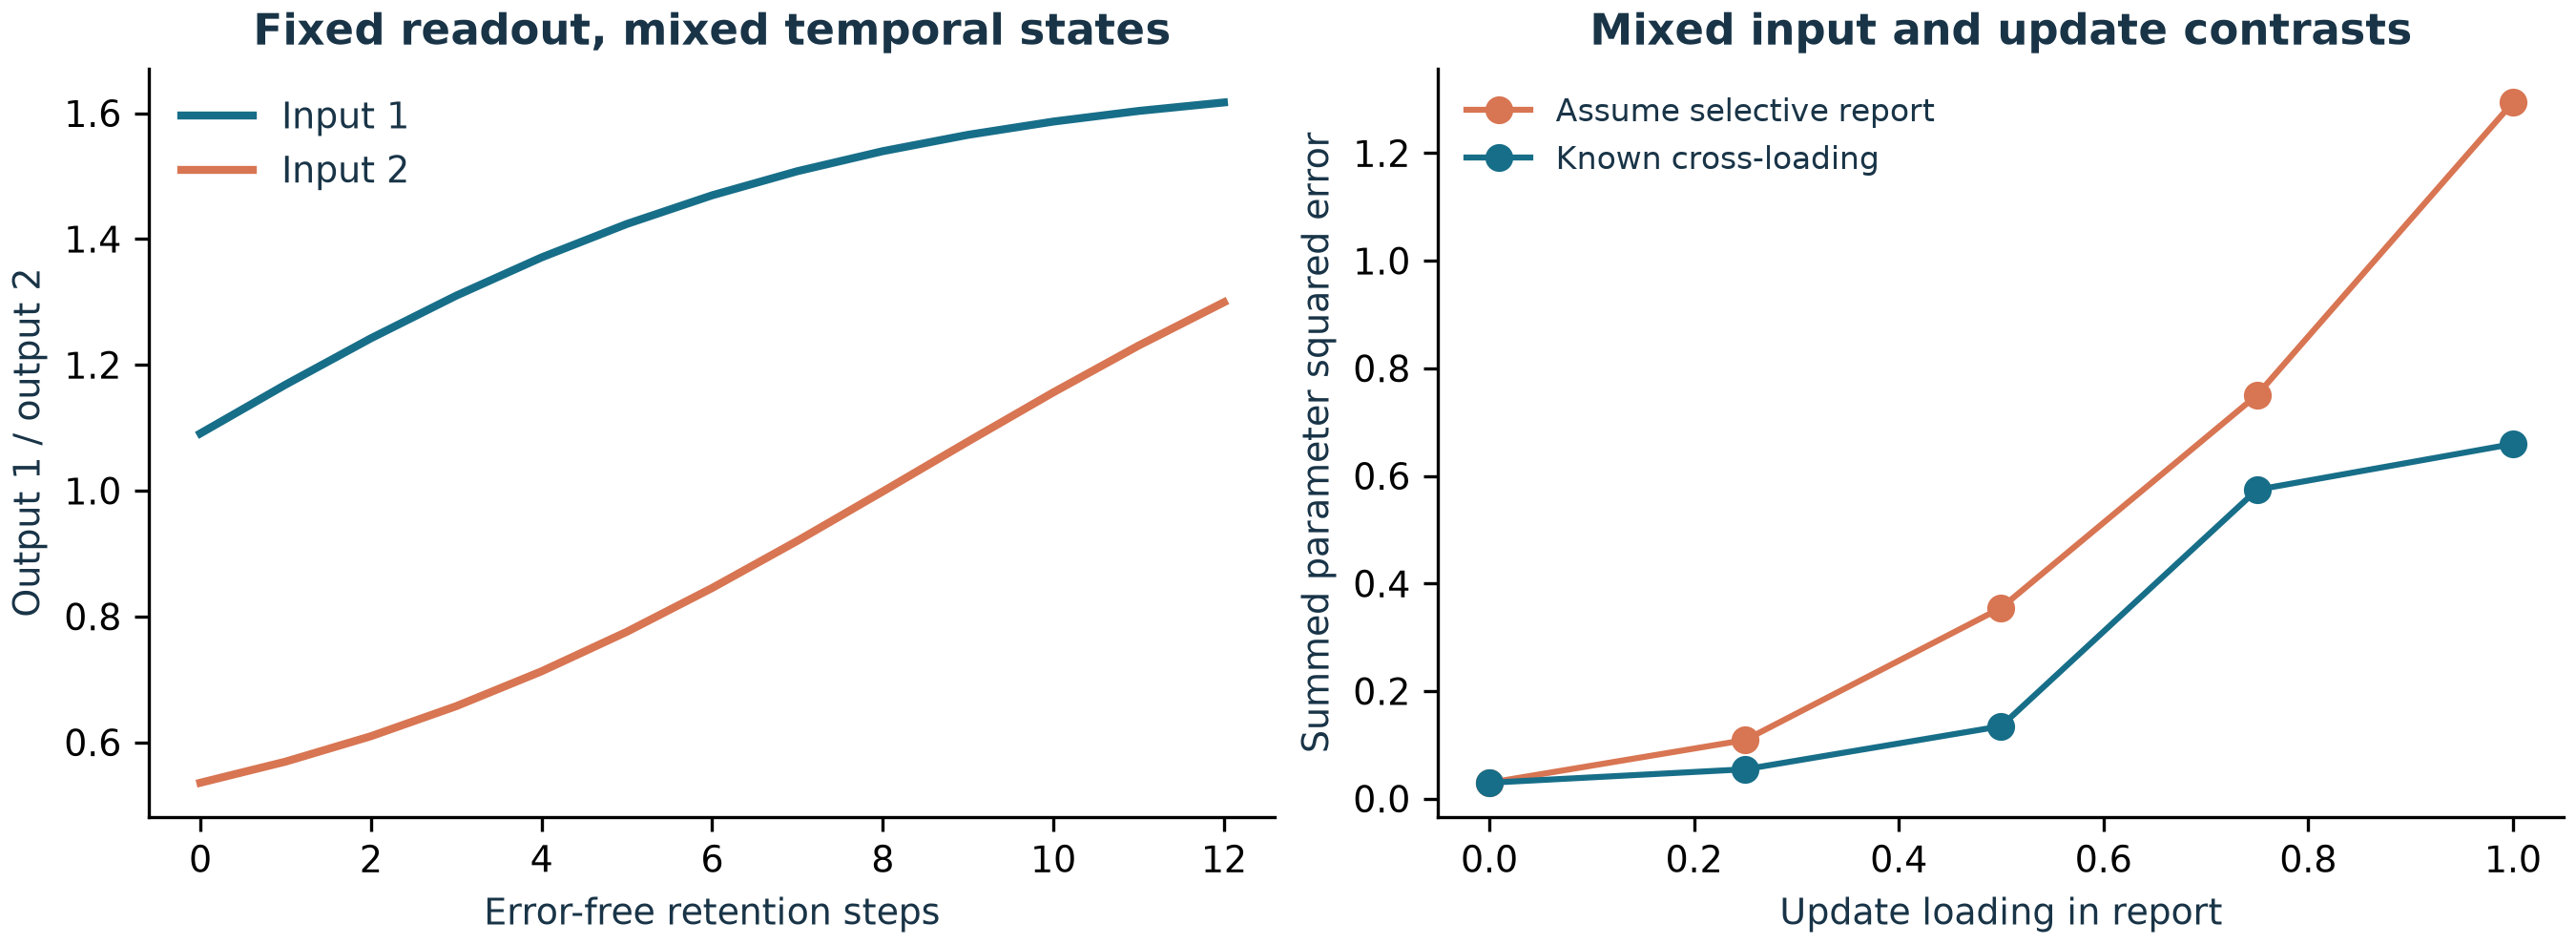
\includegraphics[width=\textwidth]{counterexamples.png}\end{center}
Left: exact fixed-readout two-mode construction. Right: pure and mixed-factor simulations under known or wrongly assumed zero report cross-loading. These are constructed examples and simulated parameter errors, separate from the human measurements. The singular case at loading one has an unresolved factor decomposition.
\clearpage\section{Noise-preserving model recovery}
Each row contains twenty fresh generating instances. Columns are forced winning labels on gradual-exposure prediction after abrupt-exposure fitting. Parameter perturbations and noise draws are new; generating families and penalty values come from the visual-error source study. The source residual library preserves paired channels and five-block segments. This is a protocol-specific diagnostic with finite Monte Carlo precision.
\begin{center}\begin{tabular}{lrrrr}\toprule True / selected & C1 & S1 & C2 & S2\\\midrule
C1 & 7 & 6 & 5 & 2\\
S1 & 6 & 4 & 6 & 4\\
C2 & 0 & 0 & 15 & 5\\
S2 & 0 & 0 & 5 & 15\\
\bottomrule\end{tabular}\end{center}
\section{Cross-loading stress: pure and mixed changes}
This test uses normalized assumed report noise SD 0.05 and factor norm 0.8, with 500 instances per cell. Parameter error sums squared errors over four input and four update coefficients. Known-loading fits and erroneous zero-loading fits use exact least squares. At loading one, the known model has rank one and its minimum-norm solution is not unique mechanistic recovery.
\small\begin{longtable}{llrrr}\toprule Loading & Truth & Wrong-model error & Known-loading error & Rank\\\midrule\endhead
0.00 & input & 0.0306 & 0.0306 & 2\\
0.00 & update & 0.0296 & 0.0296 & 2\\
0.00 & mixture & 0.0296 & 0.0296 & 2\\
0.25 & input & 0.0311 & 0.0563 & 2\\
0.25 & update & 0.1122 & 0.0537 & 2\\
0.25 & mixture & 0.1090 & 0.0546 & 2\\
0.50 & input & 0.0291 & 0.1254 & 2\\
0.50 & update & 0.3512 & 0.1299 & 2\\
0.50 & mixture & 0.3546 & 0.1346 & 2\\
0.75 & input & 0.0311 & 0.5962 & 2\\
0.75 & update & 0.7476 & 0.6036 & 2\\
0.75 & mixture & 0.7501 & 0.5742 & 2\\
1.00 & input & 0.0308 & 0.3226 & 1\\
1.00 & update & 1.3141 & 0.3224 & 1\\
1.00 & mixture & 1.2941 & 0.6593 & 1\\
\bottomrule\end{longtable}\normalsize
\section{Independent localization check}
\textbf{30implicit (n=20)} Active, passive, active-minus-passive shifts: -6.43 [-8.62, -4.04], -4.89 [-6.93, -3.12], -1.54 [-2.91, -0.12]\par
\textbf{30explicit (n=21)} Active, passive, active-minus-passive shifts: -9.01 [-11.34, -6.61], -6.63 [-9.59, -4.13], -2.38 [-4.14, -0.34]\par
\textbf{cursorjump (n=20)} Active, passive, active-minus-passive shifts: -5.68 [-7.47, -3.84], -3.85 [-5.39, -2.35], -1.84 [-3.05, -0.52]\par
\textbf{handview (n=29)} Active, passive, active-minus-passive shifts: -3.24 [-5.78, -1.11], -3.22 [-6.04, -0.82], -0.02 [-0.86, 0.81]\par
Intervals use participant resampling; all three author-interpolated spatial directions are averaged. The control/instructed groups were reused from an earlier publication and are counted once here. This reanalysis tests report selectivity within a study; it is separate from the cross-study force-field prediction.
\section{Optimization and numerical representation}
The 64-start source-only audit used a fresh random seed against the 64-start final fits. Maximum loss improvement: 1.13e-10. Close-pole divided differences avoid opposite-coefficient cancellation. Baseline-only transport scores, complete optimizer records, data hashes and source extraction checks are supplied.

\begingroup\fontsize{8.5}{9.6}\selectfont\setlength{\parskip}{0pt}\setlength{\bibsep}{0pt}\bibliographystyle{unsrtnat}\bibliography{references}\endgroup\end{document}